%% Submission to Neuromorphic Computing and Engineering (IOP Publishing)
%% Uses IOP's current template class iopjournal.cls (supplied in IOP's author kit and committed
%% alongside this file). Build:  tectonic -X compile manuscript_nce.tex
%%
%% Option [anonymous] strips author names, affiliations and acknowledgements for double-anonymous
%% review:  \documentclass[anonymous]{iopjournal}
\documentclass{iopjournal}

% Latin Modern: the Tectonic bundle lacks some Computer Modern Type 1 fonts (cmr7.pfb),
% and lmodern is a metrically compatible drop-in that the bundle does provide.
\usepackage{lmodern}
\usepackage{amsmath}
\usepackage{amssymb}
\graphicspath{{figs/}}

\begin{document}

\articletype{Paper}

\title{Short-Delay Excitatory Drive Governs Provable Silence in Recurrent Spiking Networks}

\author{[FIRST AUTHOR]$^{1,*}$\orcid{0000-0000-0000-0000}}

\affil{$^1$[DEPARTMENT, INSTITUTION, CITY, COUNTRY]}

\affil{$^*$Author to whom any correspondence should be addressed.}

\email{[CORRESPONDING EMAIL]}

\keywords{spiking neural networks, neuromorphic computing, synchronisation, synaptic delays, formal guarantees, parallel discrete-event simulation}

\begin{abstract}
Multi-core neuromorphic systems advance in discrete time steps, and before a core can compute step $t+1$ it must establish which of its presynaptic neurons spiked at step $t$. This is enforced by a global barrier or by local handshakes, and the resulting synchronisation is a recognised bottleneck. Trained recurrent spiking networks are in fact silent for most of their operation, but silence that is merely observed cannot be exploited: a core may only skip waiting if the silence of its neighbours is provable in advance. We show that provability in a recurrent spiking network is governed by a single measurable quantity: the worst-case excitatory recurrent drive arriving through synapses whose delay is shorter than the certificate horizon, denoted $R_{\mathrm{short}}$. Across six architectures spanning a twenty-fold range of $R_{\mathrm{short}}$, certified silence rises from 0\% to 98\% of the achievable maximum, monotonically in $R_{\mathrm{short}}$. Because only synapses with delay below the horizon contribute uncertainty, a network with multi-tap synaptic delays can satisfy a given $R_{\mathrm{short}}$ by relocating excitation into longer delays, leaving total excitatory mass unchanged. We observe exactly this: training with a certificate penalty reduces drive on the binding short-delay tap by 94\% while leaving total excitatory mass essentially unchanged, and the resulting networks certify 56.0\% of core-steps on the Heidelberg Spiking Digits at an accuracy change of $+0.24$ points against matched controls (three test seeds), and 61.5\% on Spiking Speech Commands at $+3.03$ points (four test seeds, frozen recipe transferred without retuning). No soundness violation occurred in any run. We further find that per-synapse learnable delays place enough mass at long lags that the unconstrained network already certifies 97.4\% of its achievable maximum, so certifiability follows from the delay distribution alone. Certificates permit barrier-free execution that is bit-identical to lock-step; in a compiled shared-memory engine this is 1.25--1.49$\times$ faster than lookahead-aware local handshaking at 32 cores, but slower below 16 cores, and in a two-process TCP configuration it is 1.37$\times$ slower, because certificates reduce waiting while leaving message count unchanged.
\end{abstract}

\section{Introduction}

Neuromorphic processors execute spiking neural networks as many small cores exchanging spike events \cite{spinnaker,truenorth,loihi}. Most advance in discrete algorithmic time steps, and the dependency is strict: before computing step $t+1$, a core must know which of its presynaptic neurons spiked at step $t$. This is enforced either by a global barrier \cite{truenorth,loihi} or by local handshakes between communicating cores \cite{neuroscale}. As systems scale, the cost of this synchronisation grows with them, and performance analyses of deployed neuromorphic workloads repeatedly identify communication and synchronisation as the limiting factor, ahead of arithmetic \cite{neuroscale,floorline,neurobench}.

Trained recurrent spiking networks offer an apparent opportunity. Their activity is sparse --- in the networks studied here the mean firing rate is around 3\% --- so cores are idle most of the time. But observed idleness cannot be exploited. A core may skip waiting for a neighbour only if that neighbour's silence is established \emph{before} the step in question; otherwise a missed spike changes the computation. The requirement is \emph{provable} sparsity. In the networks we examine, cores are genuinely silent in roughly 59\% of core-steps, and 4\% of those are provable without intervention.

This paper identifies what provability depends on. We formulate per-core silence certificates for adaptive leaky integrate-and-fire networks with multi-tap synaptic delays, and show that the certificate at horizon $k$ must bound only those synapses whose delay is \emph{shorter} than $k$; contributions arriving through longer delays originate at time steps that are already determined and can be used exactly. Provability is therefore governed by the excitation arriving through short delays, which we denote $R_{\mathrm{short}}$.

Two consequences follow, and the experiments bear out both. Longer-delay synapses are unconstrained by a horizon-$k$ certificate, so a network can reduce $R_{\mathrm{short}}$ by moving excitation into longer delays, and certifiability need not cost accuracy. Second, because the quantity is a property of the delay distribution, an architecture whose delays are naturally spread away from short lags is certifiable without any dedicated training.

Our contributions are:

\begin{enumerate}
\item \textbf{The governing quantity.} We derive the delay decomposition of the certificate and show that certified silence is monotone in $R_{\mathrm{short}}$ across six architectures spanning $R_{\mathrm{short}}$ from 0.275 to 5.983, rising from 0\% to 98\% of the achievable maximum (section~\ref{sec:governing}).
\item \textbf{Certification at no accuracy cost.} On the Heidelberg Spiking Digits, networks trained with a certificate penalty certify 56.0\% of core-steps at an accuracy change of $+0.24$ points relative to matched controls over three held-out test seeds; the recipe transferred to Spiking Speech Commands without retuning certifies 61.5\% at $+3.03$ points over four test seeds (sections~\ref{sec:shd}, \ref{sec:ssc}).
\item \textbf{Reallocation of excitation in time.} Training reduces drive on the binding short-delay tap by 94\% while total excitatory mass changes by 1--16\%, with the same signature on both datasets and every seed (section~\ref{sec:mechanism}).
\item \textbf{Certifiability as a property of the delay distribution.} With per-synapse learnable delays the \emph{unconstrained} network certifies 97.4\% of its achievable maximum; a certificate penalty is required only where the architecture does not already supply the margin (section~\ref{sec:architectural}).
\item \textbf{Exact barrier-free execution and its operating regime.} Certificates permit execution that is bit-identical to lock-step. In a shared-memory engine this runs 1.25--1.49$\times$ faster than lookahead-aware local handshaking at 32 cores and slower below 16; across two processes it runs 1.13--1.18$\times$ faster once per-message latency exceeds roughly 350\,$\mu$s and slower below it, a boundary set by the waiting it removes against the computation it adds (section~\ref{sec:execution}).
\item \textbf{Boundary conditions.} Activity-cap bounds, faster membrane leak, restricted fan-in, increased width, and learnable per-synapse delays each leave the accuracy--certifiability frontier unimproved, which delimits where the governing relation can be acted on (section~\ref{sec:negative}).
\end{enumerate}

\section{Background and related work}

\paragraph{Synchronisation in neuromorphic systems.} TrueNorth advances all cores on a global tick \cite{truenorth}. Loihi exchanges barrier messages between neighbouring cores that flush in-flight spikes and propagate the time-step advance \cite{loihi}. SpiNNaker runs cores against real-time timers and exchanges multicast packets \cite{spinnaker}. Recent work replaces global barriers with local, neighbour-to-neighbour handshakes, removing the linear growth of synchronisation cost with system size \cite{neuroscale}. Our certificates are complementary: they reduce how often a handshake must be waited for, leaving the handshake protocol itself unchanged.

\paragraph{Lookahead in parallel discrete-event simulation.} The problem of advancing a process without global synchronisation is long established. Conservative algorithms require \emph{lookahead} --- a guarantee that no event will arrive before some future time --- to let a process proceed safely \cite{fujimoto,chandymisra}; optimistic algorithms instead run ahead and roll back on causality errors \cite{jefferson}. Distributed spiking network simulators take their lookahead from the minimum synaptic delay, exchanging spikes only once per minimum-delay interval \cite{nest}. This is the structure we exploit: minimum delay supplies lookahead at no cost, and certificates extend it beyond what the delay alone provides. A baseline must therefore be given the delay-derived lookahead to be fair, and ours is throughout (section~\ref{sec:engines}).

\paragraph{Bounding spiking network dynamics.} Interval-propagation bounds on spiking network state have been used to certify robustness to input perturbation \cite{certsnn}. We use the same family of bounds for a different property --- future silence over a horizon under recurrent input --- and for a different purpose, namely making a runtime scheduling decision safe. The bounded quantity here is a temporal reach, and that is what gives rise to the delay decomposition in section~\ref{sec:decomposition}.

\paragraph{Synaptic delays in trained spiking networks.} Delays are an established route to accuracy on temporal benchmarks; methods that learn a delay per synapse reach the strongest reported results on the Heidelberg datasets \cite{dcls}. Delays also change \emph{what the certificate must bound}, and we find they make networks certifiable without a dedicated objective.

\paragraph{Event-driven reformulation of sparse spiking workloads.} A complementary line of work rewrites
time-driven spiking computations in event-driven form, so that work scales with activity rather than with
time steps; a recent example reformulates eligibility propagation this way and reports exact reductions in
computation for sparse networks, with a reference implementation in NEST \cite{eprop}. That approach
reduces the work performed under a fixed dependency structure; ours alters the dependency structure, by
making a neighbour's silence provable so the dependency need not be waited on. The two are orthogonal and
could compose.

\paragraph{Activity sparsity is not provability.} Firing-rate penalties are the standard route to sparse spiking activity. We find that sparsity and certifiability are close to orthogonal: the networks with the lowest firing rates in our sweeps are not the certifiable ones, and a strong rate penalty produces sparse networks that certify under 1\% of core-steps. The quantity that governs certifiability is the worst-case drive through short delays.

\section{Theory}

\subsection{Network model}

We consider a single recurrent layer of adaptive leaky integrate-and-fire (ALIF) neurons. With membrane potential $v$, adaptation $a$, external input $I$ and spikes $s\in\{0,1\}$, neuron $i$ evolves as
\begin{eqnarray}
a_i(t) &=& \rho\, a_i(t-1) + \gamma\, s_i(t-1) \\
v_i(t) &=& \beta\, v_i(t-1) + I_i(t) + \sum_{d\in\mathcal{D}} \sum_j W^{(d)}_{ij}\, s_j(t-d) \\
s_i(t) &=& \mathbb{1}\!\left[\, v_i(t) \ge \theta + a_i(t) \,\right],
\end{eqnarray}
followed by the reset $v_i(t) \leftarrow v_i(t) - s_i(t)\,(\theta + a_i(t))$, where $\beta=\exp(-\Delta t/\tau_m)$ is the membrane decay, $\theta$ the base threshold, and $W^{(d)}$ the recurrent weight matrix for synaptic delay $d$. Setting $\mathcal{D}=\{1\}$ recovers the conventional unit-delay recurrent network. Neurons are partitioned into $P$ cores of $C$ neurons each; a core is the unit of synchronisation.

\subsection{Silence certificates}

A core issues a certificate ``silent through step $u$'' when it can establish that none of its neurons will fire at steps $t+2,\dots,u$, whatever its neighbours do. A neighbour holding such a certificate need not be waited for over that interval. Because the true threshold $\theta + a_i$ is at least $\theta$ (adaptation is non-negative), it is sound to reason against the base threshold $\theta$.

Let $R^{(d)}_i = \sum_j \max(0, W^{(d)}_{ij})$ be the worst-case excitatory drive into neuron $i$ through delay $d$, obtained when every presynaptic neuron fires. Bounding the membrane reach forward from the measured state $v_i(t+1)$ gives a sufficient condition for silence over $K$ steps. If the drive is bounded by $R_i$ at every step, the reach converges to $R_i/(1-\beta)$, so
\begin{equation}
R_i < (1-\beta)\,\theta
\label{eq:budget}
\end{equation}
is sufficient for silence over an unbounded horizon. We refer to $(1-\beta)\theta$ as the \textbf{excitatory budget}. For the parameters used here ($\beta=e^{-1/2}$, $\theta=1$) the budget is $0.3935$. A finite-$K$ certificate is more permissive than (\ref{eq:budget}), because it starts from the measured membrane potential; section~\ref{sec:governing} quantifies the gap.

We evaluate certificates with a fixed-point refinement. Let $\mathcal{S}$ be a set of neurons that may fire within the window. Bounding each neuron's reach using only the drive attributable to $\mathcal{S}$ yields a possibly smaller set; iterating to a fixed point gives the certified set. This is sound for any initial superset and tightens the bound where the network is mostly quiet.

\subsection{The delay decomposition}
\label{sec:decomposition}

Which synapses a certificate must bound follows from arrival times. Consider a certificate rooted after step $t+1$ and a horizon $k\ge 1$, so the step under consideration is $\tau = t+1+k$. The contribution of a synapse with delay $d$ arrives from step
\begin{equation}
\tau - d = t + 1 + k - d .
\end{equation}
If $d \ge k$, then $\tau-d \le t+1$, which is a step that has \textbf{already been computed}. Its spikes are known, and the contribution can be evaluated exactly. Only synapses with $d < k$ draw on steps that are still in the future and therefore require a worst-case bound. Hence the quantity that must be bounded at horizon $k$ is
\begin{equation}
R_{\mathrm{short}}(k) = \sum_{d<k} R^{(d)}_i ,
\end{equation}
and for a $K$-step certificate the binding quantity is $R_{\mathrm{short}} = \sum_{d<K} R^{(d)}$. Two corollaries follow immediately.

First, a minimum synaptic delay $d_{\min}$ yields $d_{\min}$ steps of exact, cost-free lookahead: for $k \le d_{\min}$ no synapse satisfies $d<k$, so nothing requires bounding. This is precisely the lookahead conservative parallel simulation extracts from minimum delay \cite{fujimoto,nest}, recovered here as a special case; certificates extend lookahead beyond it.

Second, and more consequentially, $R_{\mathrm{short}}$ can be reduced \emph{without reducing total excitation}, by moving excitatory mass from short to long delays. A network with delays $\mathcal{D}=\{2,4,8\}$ and $K=4$ is bound only by its $d=2$ tap; the $d=4$ and $d=8$ taps are unconstrained by the certificate. Section~\ref{sec:mechanism} shows that trained networks exploit this. Figure~\ref{fig:mech} summarises the decomposition, the comparison a certificate makes, and what holding one licenses at run time.

\begin{figure}
\centering
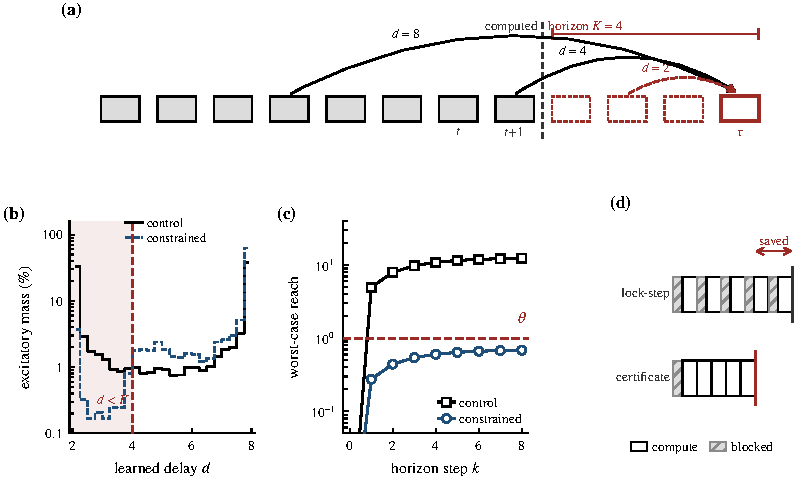
\includegraphics[width=\textwidth]{fig1_mechanism.pdf}
\caption{\label{fig:mech}Provable silence from the temporal placement of excitation. (a) A certificate rooted after step $t+1$ asks whether step $\tau=t+1+k$ can fire. A synapse of delay $d$ supplies that step from $\tau-d$: for $d \geq k$ this is a step already computed, so its contribution is known exactly, while $d<k$ draws on a step still inside the horizon and must be bounded. With $\mathcal{D}=\{2,4,8\}$ and $K=4$ only the $d=2$ tap is bounded, and the quantity that constrains the certificate is $R_{\mathrm{short}}=\sum_{d<K}R^{(d)}$. (b) Worst-case membrane reach over the horizon, $\beta^k v + R_{\mathrm{short}}(1-\beta^k)/(1-\beta)$, evaluated at the measured $R_{\mathrm{short}}$ of the control and constrained networks of table~\ref{tab:governing} with $\beta=e^{-1/2}$ and $\theta=1$. The control exceeds threshold at the first step; the constrained network stays below it for every horizon, which is what the certificate asserts. (c) What a certificate licenses: a core holding one advances through the horizon without waiting for its neighbour, instead of blocking once per step. Schematic; measured timings are in tables~\ref{tab:speed} and~\ref{tab:tcp}.}
\end{figure}

\subsection{Enforcement}

Certificates can be made to hold by adding a penalty on the worst-case $K$-step reach, evaluated on windows in which the network is in fact silent:
\begin{equation}
L = L_{\mathrm{task}} + \lambda \cdot \mathrm{mean}\!\left[\, \mathrm{relu}\!\left(\max_k \mathrm{reach}_k - \theta\right) \cdot \mathbb{1}[\mathrm{silent}] \,\right],
\end{equation}
where $\mathrm{reach}_k$ uses the exact/bounded split of section~\ref{sec:decomposition}. This is one enforcement route among several; section~\ref{sec:architectural} shows that when the delay distribution already places little mass at short lags, no penalty is needed at all.

\section{Methods}

\subsection{Datasets and protocol}

We use the Heidelberg Spiking Digits (SHD; 20 classes, 8\,156 training and 2\,264 test samples) and Spiking Speech Commands (SSC; 35 classes, 75\,466 training samples) \cite{shd}. Input spikes over 700 channels are binned into $T=100$ time steps spanning 1.4\,s.

\textbf{Selection and confirmation are strictly separated.} SHD's test set is dominated by two speakers absent from training (81.3\% of test samples come from speakers 4 and 5, which never appear in training), so a random validation split is not representative of the test condition: in earlier work on this project a configuration that won on a random split lost 4.5 accuracy points on test. All architecture and hyperparameter choices in this paper were therefore made on a \textbf{speaker-disjoint validation set} (training speakers 3 and 6 held out, 1\,169 samples), and the resulting recipe was \textbf{frozen} before any test evaluation. Reported headline results come from the frozen recipe evaluated once per run on the test set with \textbf{fresh random seeds} not used during selection. Holding out two speakers costs the control about 2.1 points of absolute test accuracy, so validation figures are systematically lower than test figures and the two are never mixed.

Every accuracy cost is computed \textbf{per seed against that seed's own matched control} --- a control with identical architecture, schedule and seed, trained without the certificate penalty --- never against a pooled control mean.

\subsection{Architectures}

All networks have $H=512$ recurrent ALIF neurons partitioned into 16 cores of 32 neurons (and 4--32 cores for the execution study), $\beta=e^{-1/2}$, $\theta=1$, $\rho=e^{-14/200}$, $\gamma=0.02$. We compare: a conventional unit-delay network ($\mathcal{D}=\{1\}$); multi-tap networks with $\mathcal{D}=\{1,2,4,8\}$ and $\mathcal{D}=\{2,4,8\}$; and a network with a learnable delay per synapse, parameterised as $D_{ij}\in[2,8]$ via a sigmoid and interpolated onto integer taps by a triangular kernel, $W^{(k)}_{ij} = W_{ij}\cdot\mathrm{relu}(1-|D_{ij}-k|)$. The interpolation kernel sums to unity per synapse, so total synaptic strength is preserved; the parameter count is $2H^2$ irrespective of the delay range, against $|\mathcal{D}|H^2$ for fixed taps.

\subsection{Training}

Surrogate-gradient training with AdamW (learning rate $2\times10^{-3}$, weight decay $10^{-4}$), batch size 128, cosine schedule, 150 epochs. Augmentation applies circular shifts in time and channel ($\pm10$ bins) and masks a random block of up to 40 channels and up to 10 time steps. Constrained networks are obtained by fine-tuning from the matched control for 150 epochs at learning rate $5\times10^{-4}$ with the penalty weight ramped linearly over the first half of training; $\lambda=1.0$ unless stated. On SSC the recipe is transferred unchanged, with the epoch count matched by \textbf{gradient steps} rather than epochs (8\,250 steps, i.e.\ 14 SSC epochs), since SSC is roughly nine times larger; this is the only adaptation made, and it was declared before the runs.

\subsection{Certification measurement}

We report the \textbf{certified core fraction}: the proportion of core-steps for which a whole core is provably silent over the next $K=4$ steps. The natural ceiling is the \textbf{oracle fraction}, the proportion of core-steps in which the core is \emph{actually} silent over the same window; a certified fraction cannot exceed it. We therefore report certification both absolutely and as a percentage of oracle. A \textbf{violation} is a certified window in which some neuron does in fact fire; violations are counted exhaustively on every evaluation and any non-zero count invalidates the corresponding result.

\subsection{Exact multi-core execution}
\label{sec:engines}

Two engines were implemented in C++20. The first is a shared-memory engine with one thread per core and emulated interconnect latency $L$, in which published data becomes visible to other cores $L$\,$\mu$s after publication. The second partitions cores across separate operating-system processes exchanging fixed-size frames over TCP with Nagle's algorithm disabled, so that latency, system-call cost and scheduling are those the operating system actually imposes.

In both engines the \textbf{baseline is given the lookahead the delays provide}: to compute step $t+1$ a core waits only for neighbour spikes up to step $t+1-d_{\min}$, which with $d_{\min}=2$ leaves every core permanently one step ahead with no certificate at all. Comparing certificates against a delay-naive handshake would attribute to the method a speed-up that belongs to the delays.

Both engines verify spike trains \textbf{bit-for-bit against a single-threaded reference} on every run. Any mismatch invalidates the timings of that run. All reported timings were taken on an otherwise idle machine; two earlier measurement attempts were discarded because concurrent workloads were detected, and in one case the idle check itself contained a race.

\section{Results}

\subsection{$R_{\mathrm{short}}$ governs certifiability}
\label{sec:governing}

The decomposition fixes, for a given horizon, exactly which synapses constrain a certificate: a tap of delay $d$ contributes to certificate step $k$ from time step $t+1+k-d$, which is already computed whenever $d \geq k$. For $\mathcal{D}=\{2,4,8\}$ a horizon of 4 therefore binds the $d=2$ tap alone, and a horizon of 8 brings $d=4$ into the binding set as well.

Re-certifying one set of trained weights at three horizons, with the weights and every other setting held fixed, follows that prediction. At $K=2$ the binding set is empty, $R_{\mathrm{short}}$ is exactly zero, and 99.2\% of the oracle fraction is certified by construction. At $K=4$ only the $d=2$ tap binds, $R_{\mathrm{short}}=0.275$, and certification reaches 94.9\% of oracle. At $K=8$ the $d=4$ tap enters the binding set, $R_{\mathrm{short}}$ rises 23-fold to 6.307, and certification falls to 0.2\% of oracle. The usable horizon is therefore bounded by the \textbf{second-smallest synaptic delay}, which makes $K=4$ the largest horizon this delay set supports. None of the 18 runs produced a soundness violation.



Table~\ref{tab:governing} compares six networks spanning a twenty-fold range of $R_{\mathrm{short}}$ on the speaker-disjoint validation set.

\begin{table}
\caption{\label{tab:governing}Certified silence is monotone in $R_{\mathrm{short}}$ and essentially independent of total recurrent excitation. Budget $(1-\beta)\theta = 0.3935$. Validation set, seed 1.}
\centering
\begin{tabular}{lrrrrrr}
\hline
architecture & accuracy & certified & oracle & \% oracle & $R_{\mathrm{short}}$ & total $R$ \\
\hline
unit delay $\mathcal{D}=\{1\}$        & 75.19 & 0.00\%  & 63.93\% & 0.0\%  & 4.840 & 4.84 \\
$\mathcal{D}=\{1,2,4,8\}$             & 81.61 & 1.63\%  & 60.11\% & 2.7\%  & 5.983 & 12.30 \\
$\mathcal{D}=\{2,4,8\}$, control      & 87.25 & 3.54\%  & 58.63\% & 6.0\%  & 4.968 & 15.27 \\
$\mathcal{D}=\{2,4,8\}$, constrained  & 87.85 & 56.28\% & 59.28\% & 94.9\% & 0.275 & 12.76 \\
learnable delays, control             & 85.54 & 55.88\% & 57.36\% & 97.4\% & 1.595 & 7.48 \\
learnable delays, constrained         & 85.63 & 55.63\% & 56.79\% & 98.0\% & 0.392 & 7.00 \\
\hline
\end{tabular}
\end{table}

\begin{figure}
\centering
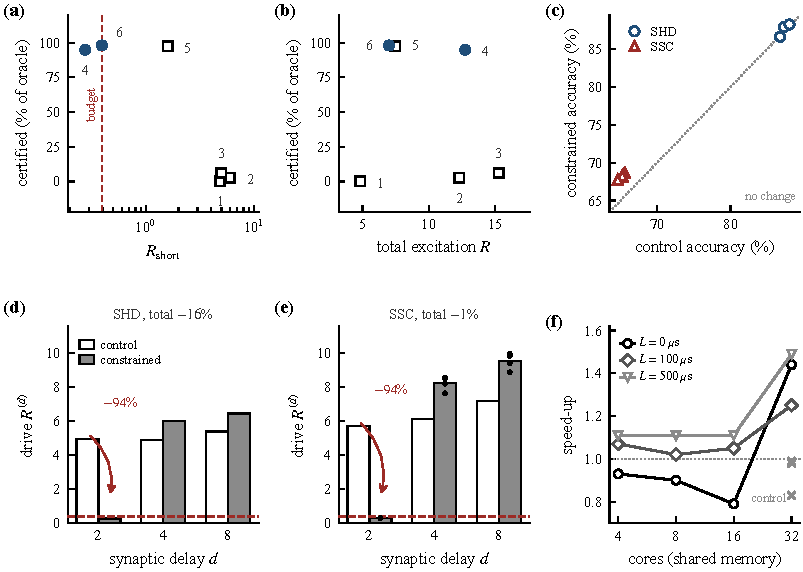
\includegraphics[width=\textwidth]{fig2_evidence.pdf}
\caption{\label{fig:evid}Measured evidence. (a) Certified silence against $R_{\mathrm{short}}$ for six architectures on the speaker-disjoint validation set: 1, unit delay $\mathcal{D}=\{1\}$; 2, $\mathcal{D}=\{1,2,4,8\}$; 3, $\mathcal{D}=\{2,4,8\}$ control; 4, $\mathcal{D}=\{2,4,8\}$ constrained; 5, learnable delays, control; 6, learnable delays, constrained. Near-oracle certification appears once $R_{\mathrm{short}}$ falls to roughly 1.6 (network 5), which is reached with and without a certificate penalty. (b) The same certified fractions against total recurrent excitation, which orders them differently and separates the governing quantity from total drive. (c) Accuracy of constrained against matched control networks on held-out test seeds, three for SHD and four for SSC; points above the diagonal cost no accuracy. (d,e) Per-tap worst-case drive before and after constrained fine-tuning: the binding $d=2$ tap falls below the excitatory budget while the unconstrained $d=4$ and $d=8$ taps grow, leaving total excitation nearly unchanged. Points in (e) are the four individual SSC test seeds. (f) Speed-up of certificate-based over lookahead-aware local handshaking in the shared-memory engine, against core count at three emulated latencies; the unconstrained control (crosses, 32 cores) gains nothing.}
\end{figure}

Certification is monotone in $R_{\mathrm{short}}$ and unrelated to total excitation (figure~\ref{fig:evid}a,b): the two networks with the largest total drive (15.27 and 12.76) sit at opposite ends of the certification range, while the pair differing only in $R_{\mathrm{short}}$ (4.968 versus 0.275) differ by a factor of sixteen in certified fraction. Near-oracle certification appears once $R_{\mathrm{short}}$ falls to roughly 1.6, about four times the budget; the finite-horizon certificate is thus more permissive than the unbounded-horizon condition (\ref{eq:budget}), as expected, since it starts from the measured membrane potential.

Core size sets how much silence is available to certify and leaves the certificate's tightness intact. Partitioning the same network into 32, 64 and 128 neurons per core certifies 56.28\%, 47.53\% and 39.92\% of core-steps against oracle fractions of 59.3\%, 50.4\% and 42.1\% --- 94.9\%, 94.2\% and 94.7\% of what is achievable. Larger cores are \emph{actually} silent less often, since certification requires every neuron in a core to be quiet; the gap between certificate and oracle does not widen.

\subsection{Certification at no accuracy cost on SHD}
\label{sec:shd}

Table~\ref{tab:shd} reports the frozen recipe evaluated once on the SHD test set with three fresh seeds.

\begin{table}
\caption{\label{tab:shd}SHD test set, frozen recipe, fresh seeds. Cost standard deviation 0.38, standard error 0.22; the 95\% interval spans roughly $-0.19$ to $+0.67$.}
\centering
\begin{tabular}{lrrrrrrr}
\hline
seed & control & constrained & cost & ctrl.\ cert.\ & cert.\ & oracle & viol.\ \\
\hline
2 & 87.28 & 87.90 & $+0.62$ & 4.08\% & 55.68\% & 58.74\% & 0 \\
3 & 86.75 & 86.62 & $-0.13$ & 4.60\% & 56.66\% & 59.44\% & 0 \\
4 & 88.03 & 88.25 & $+0.22$ & 4.06\% & 55.60\% & 58.68\% & 0 \\
\hline
mean & 87.35 & 87.59 & \textbf{+0.24} & 4.25\% & \textbf{55.98\%} & 58.95\% & \textbf{0} \\
\hline
\end{tabular}
\end{table}

Certified silence rises from 4.25\% to 55.98\%, which is 95.0\% of the oracle fraction, with no soundness violation. The accuracy change is $+0.24$ points and is statistically indistinguishable from zero. The SHD evidence supports certification at no measurable accuracy cost. An accuracy benefit appears on SSC (section~\ref{sec:ssc}), where the effect is larger than the seed spread. Selection bias from the architecture search proved small: the same configuration predicted $+0.60$ and 94.9\% of oracle on the validation set used for selection.

\subsection{Out-of-sample confirmation on SSC}
\label{sec:ssc}

The frozen SHD recipe was transferred to SSC without retuning. Table~\ref{tab:ssc} reports four test seeds.

\begin{table}
\caption{\label{tab:ssc}SSC test set, frozen recipe transferred without retuning. Cost standard deviation 0.15, standard error 0.08. Certification is 94.0\% of oracle.}
\centering
\begin{tabular}{lrrrrrrr}
\hline
seed & control & constrained & cost & ctrl.\ cert.\ & cert.\ & oracle & viol.\ \\
\hline
1 & 65.56 & 68.66 & $+3.10$ & 9.50\%  & 60.90\% & 64.59\% & 0 \\
2 & 65.25 & 68.06 & $+2.81$ & 12.94\% & 64.17\% & 68.11\% & 0 \\
3 & 65.24 & 68.33 & $+3.09$ & 11.32\% & 61.11\% & 65.21\% & 0 \\
4 & 64.61 & 67.75 & $+3.14$ & 9.51\%  & 59.73\% & 63.84\% & 0 \\
\hline
mean & 65.17 & 68.20 & \textbf{+3.03} & 10.82\% & \textbf{61.48\%} & 65.44\% & \textbf{0} \\
\hline
\end{tabular}
\end{table}

Certified silence rises from 10.82\% to 61.48\%, which is 94.0\% of oracle, with no violations. The accuracy change is $+3.03$ points with standard error 0.08 --- on this dataset the constraint acts as an effective regulariser, and the effect exceeds the seed spread by more than an order of magnitude. Absolute SSC accuracy (68.20\%) is below the strongest published results, which is expected and was stated in advance: the schedule is a step-matched transfer of an SHD recipe, with no tuning for SSC. The purpose of this experiment is to test whether the mechanism survives a change of dataset with no adaptation, and it does.

\subsection{The mechanism is reallocation, not reduction}
\label{sec:mechanism}

Table~\ref{tab:mech} shows the per-delay drive before and after constrained fine-tuning.

\begin{table}
\caption{\label{tab:mech}Training reduces drive on the binding $d=2$ tap while leaving total excitation nearly unchanged, with the same signature on both datasets and every seed.}
\centering
\begin{tabular}{lrrrr}
\hline
dataset / seed & $R^{(2)}$ & $R^{(4)}$ & $R^{(8)}$ & total \\
\hline
SHD control              & 4.97 & 4.90 & 5.40 & 15.27 \\
SHD constrained          & \textbf{0.28} & 6.03 & 6.46 & 12.76 ($-16$\%) \\
SSC control, seed 1      & 5.73 & 6.12 & 7.19 & 19.04 \\
SSC constrained, seed 1  & \textbf{0.29} & 8.56 & 9.98 & 18.83 ($-1$\%) \\
SSC constrained, seed 2  & \textbf{0.29} & 8.54 & 9.84 & --- \\
SSC constrained, seed 3  & \textbf{0.30} & 7.65 & 8.89 & --- \\
SSC constrained, seed 4  & \textbf{0.29} & 8.21 & 9.42 & --- \\
\hline
\end{tabular}
\end{table}



The binding $d=2$ tap falls by 94\% while the unconstrained $d=4$ and $d=8$ taps \emph{grow}, so total excitatory mass changes by only 1\% on SSC and 16\% on SHD (figure~\ref{fig:evid}d,e). Across four SSC seeds the $d=2$ drive lands at 0.29, 0.29, 0.30 and 0.29, and on three SHD test seeds $R_{\mathrm{short}}$ lands at 0.253, 0.253 and 0.260 --- a reproducibility of about $\pm0.01$ in the governing quantity. The constraint is satisfied by \textbf{relocating} excitation in time, which is why it costs no accuracy.

A unit-delay network shows what happens without that freedom. No longer-delay tap exists to absorb the mass, and the same budget can be met only by eliminating excitation: positive recurrent weight mass falls from 2385 to 199 (a factor of twelve) and the excitation-to-inhibition ratio from 0.650 to 0.045. Ablating recurrence in that network shows what this costs --- removing recurrent excitation costs 17.8 accuracy points in the control, while removing recurrent inhibition causes runaway firing (rate rising to 71\%) and collapse to chance. Delays give the network somewhere to put its excitation; without them, the constraint must destroy it.

\subsection{Certifiability can be architectural}
\label{sec:architectural}

The \textbf{unconstrained} learnable-delay control in table~\ref{tab:governing} certifies 55.88\% of core-steps, 97.4\% of oracle, with no certificate penalty. Adding the penalty changes certification by $-0.25$ points and accuracy by $+0.09$.

The cause is visible in the delay distribution: learned delays settle at a weighted mean of 5.04 with only 32.7\% of synapses below $d=4$, so $R_{\mathrm{short}}$ is 1.595, against the fixed-tap control's 4.968. By table~\ref{tab:governing} that difference alone is sufficient.

Certifiability is therefore a property of \textbf{where synaptic delays sit}, and a dedicated training objective is required only where the architecture does not already supply the margin. This is the more general of the two statements the evidence supports.

\subsection{Exact multi-core execution}
\label{sec:execution}

Certificates permit a core to advance without waiting for a neighbour whose certificate covers the required step. Spike trains are bit-identical to lock-step execution; this was verified against a single-threaded reference in every configuration reported below, 80 of 80 in the shared-memory engine and 54 of 54 in the TCP engine.

\begin{table}
\caption{\label{tab:speed}Speed-up of certificate-based over lookahead-aware local handshaking, shared-memory engine, idle machine. Values above 1 favour certificates. The unconstrained control gains nothing at any core count.}
\centering
\begin{tabular}{lrrrrrr}
\hline
cores & coverage & $L=0$ & $L=5$\,$\mu$s & $L=20$\,$\mu$s & $L=100$\,$\mu$s & $L=500$\,$\mu$s \\
\hline
4  & 44.5\% & 0.93 & 0.95 & 0.91 & 1.07 & 1.11 \\
8  & 52.2\% & 0.90 & 0.88 & 0.90 & 1.02 & 1.11 \\
16 & 61.5\% & 0.79 & 0.79 & 0.78 & 1.05 & 1.11 \\
\textbf{32} & \textbf{71.0\%} & \textbf{1.44} & \textbf{1.35} & \textbf{1.30} & \textbf{1.25} & \textbf{1.49} \\
32, control & 14.4\% & 0.99 & 0.98 & 0.83 & 0.98 & 0.99 \\
\hline
\end{tabular}
\end{table}



Certificate coverage rises with core count (44.5\% to 71.0\%), because certification requires a \emph{whole} core to be silent and smaller cores qualify more often; the design implication favours fine-grained many-core architectures. The unconstrained control gains nothing at any core count, which attributes the effect to training. Below 32 cores at low latency certificates \textbf{lose} (figure~\ref{fig:evid}f): their computational cost exceeds their benefit once the handshake already holds a free step from $d_{\min}=2$.

Across two processes the outcome is set by what a message costs. The engine prices messages explicitly: each frame carries its send time and becomes observable to the receiver only after a per-message latency $L$; a frame that is never sent therefore costs nothing, and $L$ prices communication while leaving computation untouched. We also record the time the main loop spends stalled on its peer. Table~\ref{tab:tcp} reports both over a range of $L$ covering loopback to $1.6$\,ms, three repeats each.

The measured computation term is independent of $L$ --- $12.9$--$14.6$\,ms for the handshake and $17.5$--$18.8$\,ms with certificates across the whole range --- which confirms that $L$ prices only communication. Certificates cost $5.1$\,ms per sample of computation at 32 cores and remove waiting that grows with $L$: $2.6$, $5.9$, $9.7$ and $18.3$\,ms at $L=200$, $400$, $800$ and $1600\,\mu$s. They pay once the waiting they remove exceeds the computation they add, which places break-even at $L\approx348\,\mu$s and matches the crossover observed between $200$ and $400\,\mu$s. Above it the advantage grows: $1.13\times$ at $L=800\,\mu$s, with min--max ranges over three repeats that do not overlap ($41.1$--$42.6$ against $46.2$--$47.3$\,ms), and $1.18\times$ at $L=1600\,\mu$s. On loopback the handshake wins by $1.35\times$, and the blocked-time measurement says why: it waits only $0.13$\,ms per sample, because $d_{\min}=2$ already supplies the lookahead it needs. Both terms of the comparison can be measured before any execution experiment, so the boundary is predictable.

A certificate also licenses a rank to stop transmitting, since a published certificate already proves the omitted steps silent. This is sound and it does reduce traffic, from $99.0$ to $71.1$ frames per sample ($1.39\times$), and it was slower than transmitting every step at every latency tested. The blocked-time measurement locates the cause: a skipping rank stalls \emph{longer} than one that transmits continuously ($26.6$ against $22.8$\,ms at $L=800\,\mu$s, in 12 of 12 repeats across four latencies). Continuous transmission keeps several frames in flight, so per-message latency overlaps local computation; omitting frames drains that pipeline, and the peer then stalls on a full latency once a spike forces a frame. The step time is set by the dependency chain, and reducing message count does not shorten it.

\begin{table}
\caption{\label{tab:tcp}Two-process TCP engine at 32 cores, median ms per sample over 100 samples, three repeats, idle machine. $L$ is the emulated per-message latency. \emph{blocked} is the time the main loop is stalled on its peer. Bold marks the faster protocol at each $L$. All 54 runs were bit-identical to the single-threaded reference.}
\centering
\begin{tabular}{rrrrrrr}
\hline
 & \multicolumn{3}{c}{total} & \multicolumn{3}{c}{blocked} \\
$L$ ($\mu$s) & handshake & cert & cert+skip & handshake & cert & cert+skip \\
\hline
0    & \textbf{13.08} & 17.59 & 17.57 & 0.13 & 0.10 & 0.10 \\
200  & \textbf{17.22} & 19.73 & 19.71 & 3.70 & 1.12 & 1.94 \\
400  & 26.71 & \textbf{26.03} & 28.01 & 13.35 & 7.43 & 8.82 \\
800  & 47.09 & \textbf{41.67} & 45.03 & 32.53 & 22.85 & 26.59 \\
1600 & 86.50 & \textbf{73.44} & 79.28 & 73.15 & 54.85 & 60.92 \\
\hline
\end{tabular}
\end{table}

\subsection{Boundary conditions}
\label{sec:negative}

Five routes suggested by the governing relation were tested and did not improve the accuracy--certifiability frontier. Each delimits where the relation can be acted on.

\begin{itemize}
\item \textbf{Tightening the bound with activity caps.} The worst-case bound assumes every presynaptic neuron fires, whereas measured simultaneous activity is 0.98 of 32 neurons per core on average (99.9th percentile 7, maximum 10) --- a pessimism factor above twenty. Yet a sound ``at most $k$ per presynaptic core'' bound tightens $R$ by only 1.1--4.1$\times$, because the positive weight distribution is heavy-tailed; even $k=1$ leaves $R$ at 1.125, still 2.9 times the budget, certifying 0\% of neurons. Activity-cap certificates therefore leave the frontier unchanged.
\item \textbf{Enlarging the budget via faster membrane leak.} The budget $(1-\beta)\theta$ grows as the membrane time constant falls, by 1.61$\times$ at $\tau_m/2$ and 2.20$\times$ at $\tau_m/4$. This raises certification but costs base accuracy, and on the delay architecture it is superseded: once delays supply the margin, the budget is no longer binding.
\item \textbf{Restricting fan-in.} $R$ is almost exactly linear in fan-in ($R \approx 0.0098 \times \mathrm{fan\text{-}in}$ across a tenfold range), so local connectivity reduces it proportionally and makes $R$ width-independent. Certification duly rises, but absolute accuracy falls by about 8 points and additional width does not recover it (65.95\% at $H=512$, 67.24\% at $H=1024$, 64.59\% at $H=2048$).
\item \textbf{Per-synapse learnable delays for accuracy.} Although they make networks certifiable without training (section~\ref{sec:architectural}), they did \textbf{not} improve accuracy: 85.54\% against the fixed-tap architecture's 87.25\%. The parameter-efficiency hypothesis --- that fixed taps were limited by their $|\mathcal{D}|H^2$ parameters --- is not supported.
\item \textbf{Longer training.} On the delay architecture 300 epochs is worse than 150 (84.69\% against 87.25\% for controls), the reverse of the delay-free case.
\end{itemize}

\section{Discussion}

\subsection{A design rule}

The results support a concrete rule. Certifiability is governed by $R_{\mathrm{short}}$, the worst-case excitatory drive arriving through synapses with delay below the certificate horizon. To obtain provable silence:

\begin{enumerate}
\item \textbf{Use synaptic delays of at least two steps and omit the unit-delay tap.} This guarantees two steps of exact lookahead and improves accuracy and certifiability together, so there is no trade-off to manage.
\item \textbf{Spread delays away from short lags.} If the delay distribution already places little excitatory mass below the horizon, certification follows with no training objective at all (section~\ref{sec:architectural}).
\item \textbf{Where a penalty is needed, expect reallocation.} Networks satisfy the constraint by moving excitation into longer delays; total excitatory mass need not fall and accuracy need not suffer.
\item \textbf{For hardware, prefer fine-grained cores.} Certification requires a whole core to be silent, so coverage rises as cores shrink (44.5\% at 4 cores to 71.0\% at 32).
\item \textbf{Compare the waiting removed against the certificate's computation.} Both are measurable, and their crossing predicts whether barrier-free execution pays on a given interconnect: at 32 cores the certificate costs $5.1$\,ms per sample and wins once per-message latency exceeds roughly $350\,\mu$s (section~\ref{sec:execution}).
\end{enumerate}

Since $R$ is linear in fan-in with a measurable coefficient, the maximum affordable fan-in for a target certification level can be computed in advance.

\subsection{Limitations}

\textbf{Absolute accuracy is below the state of the art.} Our strongest network reaches 87.59\% on SHD against roughly 96\% for the best reported architectures, and 68.20\% on SSC. The route indicated by the parameter-count evidence --- per-synapse learnable delays --- was tested and did not close it (section~\ref{sec:negative}). Depth, time resolution and training protocol were held fixed, so the remaining gap is attributable to those and is unresolved here. The evidence therefore establishes the relation over the accuracy range 85--88\% on SHD, and its behaviour at state-of-the-art accuracy would require an architecture we did not evaluate. Within the range tested the trend is favourable: the better of our two delay architectures is also the more certifiable.

\textbf{The distributed speed-up holds only above a latency threshold, measured on one configuration.} Across two processes certificates win by 1.13--1.18$\times$ above a per-message latency of roughly $350\,\mu$s and lose below it (section~\ref{sec:execution}). Two processes is the weakest distributed configuration and the engine supports no more, so both the threshold and the speed-up are established for that configuration alone; the break-even latency in particular depends on the certificate's computational cost, which scales with the number of cores per rank. Latencies above $350\,\mu$s describe commodity networked hosts and not a datacentre fabric, where microsecond round-trips would place the configuration on the losing side. The shared-memory speed-up (1.25--1.49$\times$ at 32 cores) is a separate many-core result and the two should be quoted separately. Message skipping was implemented and measured, and it does not help (section~\ref{sec:execution}).

\textbf{Latency in the shared-memory engine is emulated}, and no neuromorphic hardware was used. The TCP engine removes the emulation at the cost of supporting only two ranks.

\textbf{Scale.} Experiments use 512 recurrent neurons and up to 32 cores. The core-granularity effect in table~\ref{tab:speed} indicates that systems with far more neurons per core, as in current neuromorphic processors, certify whole cores less often; the regime in which the method pays is many fine-grained cores.

\textbf{Statistical scope.} Headline results rest on three (SHD) and four (SSC) test seeds. The architecture comparison of table~\ref{tab:governing} is single-seed on validation; its purpose is to establish the monotone relationship with $R_{\mathrm{short}}$, which spans twenty-fold and is corroborated by the multi-seed reproducibility of $R_{\mathrm{short}}$ itself ($\pm0.01$).

\textbf{One property, one optimisation.} We certify silence and use it to skip synchronisation. Whether the same approach --- training a network so that a runtime guarantee becomes provable --- extends to other properties and other exact optimisations is open, and is in our view the most interesting direction this work suggests.

\section{Conclusion}

This study establishes an operating relation between the temporal distribution of recurrent excitation and the provability of silence. The governing quantity is $R_{\mathrm{short}}$, the worst-case excitatory drive arriving through synapses whose delay falls below the certificate horizon; certified silence is monotone in it across a twenty-fold range and reaches 94--98\% of the achievable maximum once $R_{\mathrm{short}}$ falls to approximately 1.6.

The relation is actionable because the horizon partitions the synapses. Delays at or beyond the horizon arrive from steps already computed, so they carry no constraint, and a network can satisfy a given $R_{\mathrm{short}}$ by redistributing excitation in time. Trained networks do so: drive on the binding tap falls by 94\% while total excitatory mass changes by 1--16\%, with the same signature on both datasets and every seed, and the resulting networks certify 56\% of core-steps on SHD and 61\% on SSC with no soundness violation in any run. Where a delay distribution already places little mass below the horizon, the property holds with no training objective at all.

Two boundaries delimit the result. The relation was established over an accuracy range of 85--88\% on SHD, and its behaviour in networks at the reported state of the art remains open. The execution benefit is conditional, and the condition is quantitative: barrier-free execution runs faster than lookahead-aware handshaking across 32 shared-memory cores, and across two processes it wins once the waiting a certificate removes exceeds the $5.1$\,ms it costs to compute, which occurs above a per-message latency of roughly $350\,\mu$s. The quantity that governs provability is measurable before any execution experiment is run, which allows a target certification level to be converted into a constraint on fan-in and delay structure at design time.

\ack{[ACKNOWLEDGEMENTS]}

\funding{[FUNDER NAMES AND GRANT NUMBERS, or state that no funding was received]}

\roles{[AUTHOR CONTRIBUTIONS using CRediT terms: https://credit.niso.org -- e.g. Conceptualization,
Methodology, Software, Validation, Formal analysis, Investigation, Writing -- original draft,
Writing -- review and editing]}

\data{

All training, certification and execution code, the complete experimental record including pre-registered hypotheses and pass criteria for every experiment, and all result files are available at [REPOSITORY URL]. Both datasets are publicly available \cite{shd}.

}

\section*{Declaration of generative AI use}

[STATE THE JOURNAL-REQUIRED DISCLOSURE. Analysis code, experiment orchestration and manuscript drafting were carried out with the assistance of a large language model; all experimental results were produced by the code in the repository and all claims were verified against the recorded result files.]

\section*{References}

% NOTE TO CO-AUTHORS: entries marked [verify] require checking of authors, volume,
% year and venue before submission. Do not submit without checking them.
\begin{thebibliography}{99}

\bibitem{spinnaker} Furber S B, Galluppi F, Temple S and Plana L A 2014 The SpiNNaker project \textit{Proc. IEEE} \textbf{102} 652

\bibitem{truenorth} Merolla P A \textit{et al} 2014 A million spiking-neuron integrated circuit with a scalable communication network and interface \textit{Science} \textbf{345} 668

\bibitem{loihi} Davies M \textit{et al} 2018 Loihi: a neuromorphic manycore processor with on-chip learning \textit{IEEE Micro} \textbf{38} 82

\bibitem{neuroscale} [verify] Decentralised synchronisation for scalable neuromorphic systems

\bibitem{floorline} [verify] Analytical performance modelling of neuromorphic workloads identifying traffic and synchronisation bounds

\bibitem{neurobench} [verify] Yik J \textit{et al} NeuroBench: a framework for benchmarking neuromorphic computing algorithms and systems

\bibitem{fujimoto} Fujimoto R M 1990 Parallel discrete event simulation \textit{Commun. ACM} \textbf{33} 30

\bibitem{chandymisra} Chandy K M and Misra J 1979 Distributed simulation: a case study in design and verification of distributed programs \textit{IEEE Trans. Softw. Eng.} \textbf{SE-5} 440

\bibitem{jefferson} Jefferson D R 1985 Virtual time \textit{ACM Trans. Program. Lang. Syst.} \textbf{7} 404

\bibitem{nest} Gewaltig M-O and Diesmann M 2007 NEST (NEural Simulation Tool) \textit{Scholarpedia} \textbf{2} 1430

\bibitem{certsnn} [verify] Certified robustness of spiking neural networks via interval bound propagation

\bibitem{dcls} [verify] Hammouamri I, Khalfaoui-Hassani I and Masquelier T 2024 Learning delays in spiking neural networks using dilated convolutions with learnable spacings \textit{Int. Conf. on Learning Representations}

\bibitem{eprop} Korcsak-Gorzo A, Espinoza-Valverde J A, Stapmanns J, Plesser H E, Dahmen D, Bolten M, van Albada S J and Diesmann M 2026 Event-driven eligibility propagation in large sparse networks \textit{Neuromorph. Comput. Eng.} \textbf{6} 034024

\bibitem{shd} Cramer B, Stradmann Y, Schemmel J and Zenke F 2022 The Heidelberg spiking data sets for the systematic evaluation of spiking neural networks \textit{IEEE Trans. Neural Netw. Learn. Syst.} \textbf{33} 2744

\bibitem{lsnn} Bellec G, Salaj D, Subramoney A, Legenstein R and Maass W 2018 Long short-term memory and learning-to-learn in networks of spiking neurons \textit{Advances in Neural Information Processing Systems} \textbf{31}

\bibitem{asrnn} Yin B, Corradi F and Boht\'e S M 2021 Accurate and efficient time-domain classification with adaptive spiking recurrent neural networks \textit{Nat. Mach. Intell.} \textbf{3} 905

\end{thebibliography}

\end{document}
